\chapter{Estado del arte}
\label{estado_del_arte}

\section{Imágenes SAR y la generación de ruido \emph{speckle}}

\subsection{Fundamentos de la tecnología SAR}

Las imágenes SAR (Synthetic Aperture Radar) representan una de las tecnologías más avanzadas en teledetección activa, capaz de operar independientemente de las condiciones atmosféricas y de iluminación. Estos sistemas se obtienen mediante sensores activos que emiten ondas electromagnéticas en el rango de las microondas (típicamente entre $1$cm y $1$m de longitud de onda) y miden la señal reflejada por la superficie terrestre \cite{moreira2013tutorial}. La tecnología SAR ha evolucionado mucho desde sus primeras implementaciones en la década de 1950, convirtiéndose en una herramienta indispensable para aplicaciones como el monitoreo ambiental, la agricultura de precisión, la gestión de desastres naturales, y aplicaciones de defensa \cite{cumming2005digital}.

El proceso de formación de imágenes SAR se basa en el principio de síntesis de apertura, donde el movimiento del sensor a lo largo de su trayectoria permite simular una antena de gran tamaño, mejorando así la resolución azimutal de la imagen. Las imágenes se generan a partir de la información compleja de fase y amplitud de las ondas reflejadas, lo cual permite construir imágenes de alta resolución espacial que pueden alcanzar resoluciones muy buenas en sistemas modernos como TerraSAR-X o COSMO-SkyMed \cite{werninghaus2010terrasar}. La información de fase es particularmente valiosa para aplicaciones interferométricas (InSAR), permitiendo la detección de cambios muy pequeños en la superficie terrestre \cite{rosen2000synthetic}.

En la Figura \ref{fig:imagenes_sar_ruido} se presentan dos ejemplos de imágenes SAR reales que ilustran la complejidad y de estas representaciones. La primera imagen (Figura \ref{Sanfran}) muestra la bahía de San Francisco, CA, USA, donde se pueden observar claramente las estructuras urbanas, los puentes, y la línea costera. La segunda imagen (Figura \ref{Munich}) corresponde a los alrededores de la ciudad de Múnich, Alemania, donde se aprecia la mezcla de zonas urbanas, agrícolas y forestales, cada una con características distintivas de backscatter.

\begin{figure}[htbp]
	\vspace{0.3cm}
	\centering
	\begin{subfigure}[b]{0.48\textwidth}
		\centering
		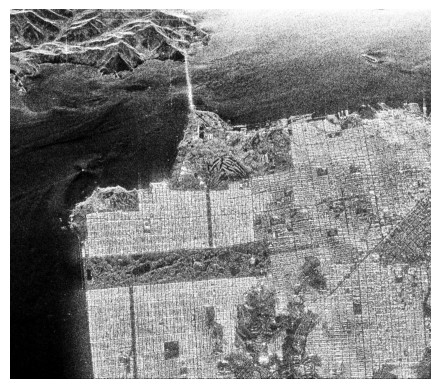
\includegraphics[height=6.9cm]{Images/sar_sanfran.jpg}
		\caption{Bahía de San Francisco, CA, EEUU.}
		\label{Sanfran}
	\end{subfigure}
	\hfill
	\begin{subfigure}[b]{0.48\textwidth}
		\centering
		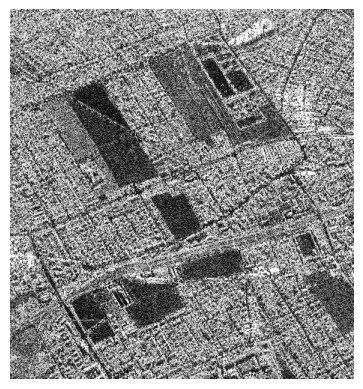
\includegraphics[height=6.9cm]{Images/sar_munich.jpg}
		\caption{Ciudad de Múnich, Alemania.}
		\label{Munich}
	\end{subfigure}
	\caption{Ejemplo de imágenes SAR con ruido reales.}
	\label{fig:imagenes_sar_ruido}
\end{figure}

\subsection{Naturaleza y características del ruido \emph{speckle}}

Una de las características distintivas y más desafiantes del ruido en imágenes SAR es su naturaleza multiplicativa, a diferencia del ruido aditivo gaussiano común en imágenes ópticas \cite{argenti2013tutorial}. Este fenómeno se origina debido a la coherencia de la señal del radar y la interferencia constructiva y destructiva de las ondas reflejadas \cite{goodman2007speckle}. Matemáticamente, el modelo de ruido multiplicativo puede expresarse como:

\begin{equation}
	I = R \cdot n,
\end{equation}
donde $I$ es la intensidad observada, $R$ es la reflectividad real de la superficie (la señal libre de ruido que queremos recuperar), y $n$ es el término de ruido multiplicativo \emph{speckle}. Esto significa que el ruido no se suma a la señal, sino que se multiplica por ella, amplificándose en las zonas de mayor intensidad (mayor retorno de señal) y siendo menos notable en las regiones más oscuras. Como consecuencia directa, este tipo de ruido genera una textura granular característica que dificulta significativamente la interpretación visual de la imagen, la detección automática de objetivos, y la aplicación de técnicas de procesamiento de imágenes convencionales \cite{touzi2002review}.

El ruido \emph{speckle} presenta propiedades estadísticas complejas que varían según el tipo de superficie observada y las condiciones de adquisición. Esto complica su modelización y torna más interesante este problema.

\subsection{Física del backscatter y su relación con el ruido}

La señal que regresa al sensor después de interactuar con la superficie terrestre es conocida como \emph{backscatter} o retrodispersión, y constituye la base fundamental para construir la intensidad de píxeles en la imagen SAR. El coeficiente de \emph{backscatter} representa la cantidad de energía reflejada por unidad de área y es una medida normalizada que permite comparaciones entre diferentes sistemas SAR y condiciones de adquisición \cite{ulaby2014microwave}.

El valor del \emph{backscatter} varía considerablemente según múltiples propiedades físicas de la superficie observada. Entre los factores más influyentes se encuentran:

\begin{itemize}
	\item \textbf{Rugosidad superficial}: La rugosidad relativa a la longitud de onda del radar determina si la reflexión es especular (superficies lisas) o difusa (superficies rugosas). El criterio de Rayleigh establece que una superficie se considera lisa si $h < \lambda/(8\cos\theta)$, donde $h$ es la altura RMS de las irregularidades (es decir, la desviación cuadrática media de las alturas respecto al promedio de la superficie), $\lambda$ es la longitud de onda y $\theta$ es el ángulo de incidencia \cite{fung2019microwave}.
	
	\item \textbf{Constante dieléctrica}: El contenido de humedad en el suelo o la vegetación afecta significativamente la constante dieléctrica del material, lo que a su vez modifica la intensidad del \emph{backscatter}. Suelos húmedos típicamente presentan valores de \emph{backscatter} entre 3 y 5 decibeles (dB) mayores que suelos secos \cite{dubois1995measuring}, donde el decibel es una escala logarítmica utilizada para medir la intensidad relativa de la señal reflejada.
	
	\item \textbf{Geometría de adquisición}: El ángulo de incidencia local, que depende tanto del ángulo de observación del sensor como de la topografía local, tiene un impacto directo en la intensidad del \emph{backscatter}. Ángulos de incidencia menores generalmente resultan en mayor \emph{backscatter} para la mayoría de las superficies naturales \cite{freeman1992calibration}.
	
	\item \textbf{Polarización}: La configuración de polarización (HH, VV, HV, VH) indica si la onda transmitida y recibida es horizontal (H) o vertical (V); HH y VV corresponden a co-polarizaciones, mientras que HV y VH a despolarizaciones. La despolarización ocurre cuando la señal cambia de polarización al interactuar con los objetos, fenómeno típico de un \emph{volumen de scattering} (dispersión en un medio con muchos elementos tridimensionales, como vegetación densa), lo que permite distinguir entre reflexiones especulares de superficies lisas y dispersión difusa propia de coberturas vegetales \cite{cloude1997entropy}.
\end{itemize}

En general, superficies rugosas o con estructuras complejas, como áreas urbanas con múltiples reflexiones o vegetación densa con \emph{scattering} volumétrico, generan un mayor ruido \emph{speckle} debido a la mayor variabilidad en las contribuciones de fase de los dispersores individuales. Por el contrario, superficies lisas como cuerpos de agua en calma actúan como reflectores especulares, desviando la mayor parte de la señal en dirección opuesta al sensor (\emph{forward scattering}), lo que resulta en valores de \emph{backscatter} muy bajos y aparecen como áreas oscuras en la imagen \cite{lee2009polarimetric}.

\subsection{Procesamiento multi-look y reducción del \emph{speckle}}

En el ámbito del procesamiento de imágenes SAR, el número de \emph{looks} representa un concepto fundamental para la comprensión y mitigación del ruido \emph{speckle}. El procesamiento multi-\emph{look} es una técnica estándar que reduce el ruido mediante el promediado de múltiples observaciones estadísticamente independientes (o \emph{looks}) de una misma área \cite{porcello1976speckle}. 

Estas observaciones independientes pueden generarse mediante diferentes estrategias:

\begin{itemize}
	\item \textbf{División espectral}: El ancho de banda del sistema se divide en sub-bandas que se procesan independientemente. Cada sub-banda produce una imagen con resolución degradada pero con \emph{speckle} independiente \cite{brusch2011ship}.
	
	\item \textbf{División espacial}: La apertura sintética, que es la distancia que recorre el radar mientras toma datos, se divide en sub-aperturas, cada una generando una imagen independiente con menor resolución azimutal \cite{fattahi2017insar}.
	
	\item \textbf{Promediado temporal}: En aplicaciones con adquisiciones repetidas de la misma área, se pueden promediar imágenes tomadas en diferentes tiempos, asumiendo que la escena permanece estable \cite{quegan2001filtering}.
\end{itemize}

El procesamiento multi-\emph{look} reduce la varianza del \emph{speckle} por un factor igual al número de \emph{looks} $L$, siguiendo la relación $\sigma_L^2 = \sigma_1^2\big/L$, donde $\sigma_L^2$ es la varianza del \emph{speckle} de $L$ \emph{looks}. Sin embargo, esta mejora en la calidad radiométrica viene acompañada de una pérdida proporcional en la resolución espacial, estableciendo un compromiso fundamental en el procesamiento SAR \cite{lopez1990adaptive}.

Para cuantificar objetivamente este balance entre reducción de ruido y preservación de resolución, se utiliza el concepto de Número Equivalente de \emph{Looks} (ENL - Equivalent Number of Looks). El ENL es una medida estadística que estima la efectividad del procesamiento multi-\emph{look} o de cualquier técnica de filtrado, definido como:

\begin{equation}
	\text{ENL} = \frac{\mu^2}{\sigma^2},
\end{equation}
donde $\mu$ y $\sigma^2$ son la media y la varianza de la intensidad en una región homogénea, respectivamente. Un valor de ENL alto indica una imagen más homogénea con menor presencia de ruido \emph{speckle}, mientras que un valor bajo sugiere mayor contaminación por ruido. Para \emph{speckle} completamente desarrollado en imágenes de intensidad de un solo look, el ENL teórico es 1, mientras que para $L$ looks independientes, el ENL teórico es $L$ \cite{anfinsen2009estimation}. Este parámetro es ampliamente utilizado para evaluar la calidad de las imágenes SAR procesadas y comparar la efectividad de distintos métodos de reducción de ruido.

\subsection{Modelado estadístico del ruido \emph{speckle}}

El modelado preciso del ruido \emph{speckle} es fundamental para el desarrollo de técnicas efectivas de filtrado y para la simulación realista de imágenes SAR sintéticas. A lo largo de las décadas, se han propuesto diversos modelos estadísticos, cada uno con sus ventajas y limitaciones específicas.

\subsubsection{Modelos clásicos de distribución}

Uno de los métodos clásicos más utilizados para generar imágenes sintéticas con ruido \emph{speckle} es el uso de la distribución Gamma ($\Gamma$). Para imágenes multi-\emph{look}, la función de densidad de probabilidad (PDF) de la distribución Gamma está dada por:

\begin{equation}
	p(I) = \frac{L^L}{\Gamma(L)\mu^L} I^{L-1} \exp\left(-\frac{LI}{\mu}\right),
\end{equation}
donde $L$ es el número de \emph{looks}, $\mu$ es la intensidad media, y $\Gamma(\cdot)$ es la función gamma \cite{gao2010statistical}. Este modelo es particularmente efectivo para áreas homogéneas pero presenta limitaciones en regiones heterogéneas.

La distribución de Rayleigh, aunque más simple, solo es efectiva para modelar la amplitud en superficies homogéneas con gran número de dispersores, típicamente superficies de pastura o agrícolas \cite{jakeman1976model}. Su PDF para la amplitud está dada por:

\begin{equation}
	p(A) = \frac{A}{\sigma^2} \exp\left(-\frac{A^2}{2\sigma^2}\right),
\end{equation}
donde $A$ es la amplitud y $\sigma^2$ es el parámetro de escala, que determina la dispersión de la distribución: valores mayores de $\sigma^2$ corresponden a amplitudes promedio más altas, mientras que valores menores concentran la amplitud cerca de cero.

Para superficies más complejas, se han desarrollado modelos como la distribución K \cite{jao1984amplitude}, que combina las fluctuaciones del \emph{speckle} con la variabilidad del terreno mediante un modelo compuesto:

\begin{equation}
	p(I) = \frac{2}{\Gamma(L)\Gamma(\nu)}\left(\frac{L\nu}{\mu}\right)^{(L+\nu)/2} I^{(L+\nu)/2-1} K_{\nu-L}\left(2\sqrt{\frac{L\nu I}{\mu}}\right),
\end{equation}
donde $K_v$ es la función de Bessel modificada de segunda especie y $\nu$ es el parámetro de forma que controla la heterogeneidad del terreno.

\subsubsection{La distribución $\mathcal{G}_I^0$ y sus ventajas}

La distribución $\mathcal{G}_I^0$, introducida por Frery et al. \cite{originalGI0}, representa uno de los avances más significativos en el modelado estadístico del \emph{speckle} en imágenes SAR. Esta distribución es particularmente versátil para generar ruido \emph{speckle}, ya que puede modelar desde áreas extremadamente homogéneas hasta regiones altamente heterogéneas mediante el ajuste de sus parámetros.

La PDF de la distribución $\mathcal{G}_I^0$ para la intensidad está dada por:

\begin{equation}
	p_I(z) = \frac{L^L \Gamma(L-\alpha)}{\gamma^\alpha \Gamma(L)\Gamma(-\alpha)} \frac{z^{L-1}}{(\gamma + Lz)^{L-\alpha}},
\end{equation}
donde $L\geq 1$ es el número de \emph{looks}, $\alpha < 0$ es el parámetro de rugosidad (valores más negativos indican mayor homogeneidad), y $\gamma>0$ es el parámetro de escala. La flexibilidad de este modelo radica en que:

\begin{itemize}
	\item Para $\alpha \to -\infty$, la distribución converge a la distribución $\Gamma$ (áreas homogéneas).
	\item Para valores intermedios de $\alpha$, modela áreas con heterogeneidad moderada (bosques, zonas agrícolas).
	\item Para $\alpha$ cercano a 0, representa áreas extremadamente heterogéneas (zonas urbanas).
\end{itemize}

Esta versatilidad hace que la distribución $\mathcal{G}_I^0$ sea ideal para la generación de datasets sintéticos de entrenamiento para algoritmos de \emph{deep learning}, permitiendo simular una amplia variedad de condiciones \cite{gomez2017unassisted}.

Trabajos recientes han extendido el modelo $\mathcal{G}_I^0$ para incluir correlación espacial \cite{bustos2002simulation} y para datos polarimétricos \cite{doulgeris2011automated}, aumentando aún más su aplicabilidad. Wang et al. \cite{wang2017sar} aplican enfoques estadísticos propios para simular el ruido, aunque requieren conocimiento previo de características específicas del mismo, lo que limita su generalización.

\subsubsection{Modelos basados en física}

Además de los modelos puramente estadísticos, existen modelos de simulación basados en la física del proceso de adquisición de imágenes SAR. El modelo IEM (Integral Equation Model) \cite{fung1992backscattering} simula la interacción de las ondas electromagnéticas con la superficie terrestre resolviendo las ecuaciones de Maxwell bajo ciertas aproximaciones. Este modelo puede predecir el \emph{backscatter} basándose en parámetros físicos como la rugosidad superficial, la constante dieléctrica, y la geometría de observación. Sin embargo, el modelo IEM presenta limitaciones significativas:
\begin{itemize}
	\item Validez limitada a superficies con rugosidad moderada.
	\item Dificultad para simular superficies con características complejas y heterogéneas.
	\item Alto costo computacional para simulaciones de grandes áreas.
	\item Necesidad de parámetros de entrada detallados que no siempre están disponibles.
\end{itemize}

Modelos más avanzados como el AIEM (Advanced IEM) \cite{chen2003note} y métodos numéricos como FDTD (\emph{Finite-Difference Time-Domain}) \cite{tsang2004scattering} ofrecen mayor precisión pero a costa de una complejidad computacional prohibitiva para aplicaciones prácticas de procesamiento de imágenes.

\section{Filtros clásicos para la reducción del ruido \emph{speckle}}

\subsection{Filtros adaptativos locales}

Los métodos clásicos para la eliminación de ruido \emph{speckle} en imágenes SAR han sido fundamentales en el desarrollo del campo y continúan siendo ampliamente utilizados debido a su eficiencia computacional y fundamentos teóricos sólidos.

\subsubsection{Filtro de Lee}\label{sec:descripcion_filtro_lee}

El filtro de Lee \cite{lee1980digital}, uno de los primeros y más influyentes en el campo, es un método clásico de filtrado no lineal ampliamente utilizado en el procesamiento de imágenes con ruido \emph{speckle}. Se basa en un enfoque de mínimos cuadrados que busca minimizar el error cuadrático medio dentro de una ventana local deslizante para estimar el valor libre de ruido. Opera aplicando la siguiente ecuación:

\begin{equation}
	\hat{R}(x,y) = \bar{I} + k(I(x,y) - \bar{I}),
\end{equation}
donde $\hat{R}(x,y)$ es la estimación del píxel filtrado, $I(x,y)$ es el valor observado, $\bar{I}$ es la media local, y $k$ es el factor de peso adaptativo dado por:

\begin{equation}
	k = \frac{\text{var}(I) - \bar{I}^2\sigma_n^2}{\text{var}(I)(1 + \sigma_n^2)},
\end{equation}
donde $\sigma_n^2$ es la varianza estimada del ruido \emph{speckle}, que debe proporcionarse como \emph{input}. El filtro calcula un promedio ponderado de los píxeles en una vecindad, ajustando el nivel de suavizado según el contraste local: suaviza fuertemente en regiones homogéneas y preserva los detalles en áreas con bordes o alta variación. Sin embargo, su desempeño depende del tamaño de la ventana de filtrado, que debe seleccionarse manualmente, y puede generar halos en zonas de transición abrupta, como en la interfaz entre agua y tierra.

El filtro de Lee ha sido extendido en múltiples variantes, incluyendo el \emph{Enhanced Lee filter} \cite{lopes1990structure}, que mejora la preservación de bordes mediante la incorporación de detectores de características.

\subsubsection{Filtro de Frost}

El filtro de Frost \cite{frost1982model} adopta un enfoque diferente, utilizando un kernel adaptativo exponencialmente ponderado que responde a la variación local de la escena:

\begin{equation}
	\hat{R}(x,y) = \sum_{(a,b) \in W} K(a,b) \cdot I(a,b).
\end{equation}
Aquí, $I(a,b)$ representa el valor del píxel en la posición $(a,b)$, que se encuentra dentro de la ventana o vecindad $W$ centrada en el píxel $(x,y)$. Los índices $a$ y $b$ recorren todos los píxeles dentro de esa vecindad, por ejemplo, una ventana de tamaño 3x3, 4x4, o 5x5. El kernel $K(a,b)$ está dado por:

\begin{equation}
	K(a,b) = K_0 \exp(-\alpha \cdot CV^2 \cdot d(a,b)),
\end{equation}
siendo $CV$ el coeficiente de variación local, $d(a,b)$ la distancia desde el píxel central $(x,y)$, y $\alpha$ un parámetro de amortiguamiento. Este filtro es particularmente efectivo en la preservación de características lineales y puntuales, ya que los píxeles cercanos al centro de la ventana tienen mayor peso y los píxeles en regiones homogéneas se suavizan más fuertemente.

\subsubsection{Filtro de Kuan}

El filtro de Kuan \cite{kuan1987adaptive} es similar al de Lee pero deriva del criterio de Minimum Mean Square Error (MMSE) bajo un modelo de ruido multiplicativo. Su formulación es:

\begin{equation}
	\hat{R}(x,y) = \bar{I} + \frac{W}{1+W}(I(x,y) - \bar{I}),
\end{equation}
donde $W = (1 - C_u^2/C_I^2)$, siendo $C_u$ el coeficiente de variación del ruido y $C_I$ el coeficiente de variación de la imagen observada.

\subsubsection{Filtros MAP}

Los filtros MAP (Maximum A Posteriori) \cite{lopes1993maximum} representan un enfoque más sofisticado que incorpora información estadística a priori sobre la distribución del \emph{backscatter}. Estos filtros utilizan estimación bayesiana para maximizar la probabilidad a posteriori:

\begin{equation}
	\hat{R} = \arg\max_R P(R|I) = \arg\max_R P(I|R) \cdot P(R).
\end{equation}
El filtro Gamma-MAP \cite{lopes1993maximum}, por ejemplo, asume una distribución $\Gamma$ tanto para el \emph{speckle} como para el \emph{backscatter}, resultando en una solución analítica cerrada. Sin embargo, la principal limitación de estos filtros adaptativos locales es que pueden generar cierto grado de borrosidad en la imagen, especialmente en áreas con alta densidad de características, llevando a la pérdida de detalles estructurales importantes.

\subsection{Filtros basados en transformadas}

Los métodos basados en transformadas matemáticas ofrecen una perspectiva diferente para el filtrado del \emph{speckle}, operando en dominios transformados donde la señal y el ruido presentan características distinguibles.

\subsubsection{Métodos basados en Wavelets}

La transformada wavelet ha demostrado ser particularmente efectiva para el despeckling debido a su capacidad de análisis multiresolución \cite{argenti2002speckle}. El proceso general involucra:

\begin{enumerate}
	\item Aplicación de la transformada wavelet logarítmica para convertir el ruido multiplicativo en aditivo.
		\item Umbralización de los coeficientes wavelet, la cual puede realizarse mediante dos estrategias principales:
	\begin{itemize}
		\item \emph{Hard thresholding}: elimina bruscamente los coeficientes cuya magnitud es menor que un umbral, conservando sin cambios los restantes.
		\item \emph{Soft thresholding}: además de anular los coeficientes pequeños, reduce gradualmente la magnitud de los grandes, generando una transición más suave.
	\end{itemize}
	\item Transformada inversa y exponenciación.
\end{enumerate}

El método de wavelets discreto \cite{zhang2017nonmodel} utiliza funciones de umbralización adaptativas que consideran las propiedades estadísticas locales del \emph{speckle}. El procedimiento se basa en la siguiente regla de umbralización suave (\emph{soft thresholding}):

\begin{equation}
	\hat{w} = \begin{cases} 
		\text{sign}(w)(|w| - T) & \text{si } |w| > T, \\
		0 & \text{si } |w| \leq T,
	\end{cases}
\end{equation}
donde $w$ es un coeficiente wavelet, $\hat{w}$ es el coeficiente procesado, $\text{sign}(w)$ representa el signo de $w$, y $T$ es el umbral adaptativo. Dicho umbral se calcula comúnmente como:

\begin{equation}
	T = \sigma_n \sqrt{2\log N},
\end{equation}
siendo $\sigma_n$ la desviación estándar del ruido y $N$ el número total de coeficientes en la descomposición wavelet. De este modo, los coeficientes pequeños (principalmente asociados al ruido) se anulan, mientras que los más grandes se reducen suavemente en magnitud, preservando los detalles estructurales de la imagen.

Trabajos más recientes han explorado wavelets no decimadas \cite{argenti2004speckle} y wavelets adaptativas \cite{ranjani2010dual} para mejorar la preservación de detalles. En particular, la transformada wavelet estacionaria (SWT) corresponde a una variante no decimada en la cual no se realiza un submuestreo tras la filtración, manteniendo el mismo número de coeficientes en cada nivel. Esto evita los artefactos de aliasing asociados con la transformada wavelet discreta tradicional (DWT) y ofrece mayor robustez frente a traslaciones, a costa de una representación redundante.

\subsubsection{Transformada de Contourlet y Shearlet}

El método de Shearlet \cite{hou2012shearlet} extiende las capacidades de las wavelets al ofrecer una mejor representación de características direccionales, permitiendo capturar información en múltiples orientaciones, y al incorporar anisotropía, adaptando la forma y escala del análisis a estructuras elongadas o con orientación preferencial. A diferencia de las wavelets tradicionales, que realizan un análisis multiescala isotrópico, las shearlets introducen transformaciones de corte (\emph{shear}) que permiten capturar bordes y estructuras orientadas con mayor precisión. 

Para la eliminación de ruido speckle, la transformada Shearlet no submuestreada (NSST) explota la diferencia en el comportamiento estadístico entre el ruido y las características de la imagen en el dominio transformado. El ruido \emph{speckle}, al ser multiplicativo y de naturaleza granular, se distribuye de manera relativamente uniforme a través de las diferentes escalas y orientaciones, mientras que las características reales de la imagen (bordes, texturas) presentan una concentración de energía en coeficientes específicos. Este principio permite aplicar estrategias de umbralización adaptativa: los coeficientes de baja magnitud, típicamente asociados al ruido, son suprimidos o atenuados, mientras que los coeficientes de alta magnitud, correspondientes a estructuras genuinas de la imagen, son preservados.

La función generadora de Shearlet se define como:

\begin{equation}
	\psi_{a,s,t}(x) = a^{-3/4}\,\psi\!\left(A_a^{-1}S_s^{-1}(x-t)\right),
\end{equation}
donde $a$ controla la escala, $s$ ajusta la orientación, $t$ corresponde a la traslación, $A_a$ es la matriz de escalado anisotrópico y $S_s$ la matriz de corte. Esta formulación permite representar de manera más eficiente contornos y bordes orientados, superando las limitaciones de las wavelets convencionales.

La transformada de Contourlet \cite{po2006directional}, otra extensión direccional de wavelets, utiliza un conjunto de filtros direccionales junto con una pirámide laplaciana (una estructura multiescala que descompone la imagen en diferentes niveles de detalle) para capturar contornos de manera eficiente. Estos métodos son particularmente efectivos para imágenes con estructuras geométricas dominantes, comunes en áreas urbanas.

Su aplicación al problema de \emph{despeckling} sigue un esquema de tres pasos: (1) descomposición de la imagen SAR ruidosa en coeficientes de Contourlet, (2) modificación de los coeficientes mediante técnicas de umbralización (hard, soft, o adaptativa) basadas en modelos estadísticos del ruido \emph{speckle}, y (3) reconstrucción de la imagen mediante la transformada inversa. La ventaja clave es que la representación direccional permite preservar mejor los contornos y estructuras geométricas durante el proceso de eliminación del ruido, evitando el suavizado excesivo característico de filtros isotrópicos.

\subsubsection{Transformada de Curvelet}

Esta transformada \cite{starck2002curvelet} ofrece una representación óptima para objetos con singularidades a lo largo de curvas, proporcionando una tasa de aproximación superior a las wavelets para este tipo de características. En el contexto de eliminación de \emph{speckle} en imágenes SAR, las curvelets son particularmente efectivas porque muchas características en estas imágenes (líneas de costa, rutas, límites de parcelas agrícolas) presentan geometrías curvilíneas que son capturadas eficientemente por esta transformada.

Una curvelet localizada se define como:

\begin{equation}
	\gamma_{\mu}(x) = \gamma(R_\theta(x - x_\mu)),
\end{equation}
donde $\gamma$ es la función base o \emph{curvelet madre}, $R_\theta$ representa una rotación por un ángulo $\theta$ que ajusta la orientación, y $x_\mu$ corresponde a la traslación espacial. De esta forma, cada curvelet se adapta tanto en posición como en dirección, lo que permite capturar de manera eficiente bordes curvos y estructuras geométricas.

El proceso de \emph{despeckling} mediante curvelets aprovecha que el ruido y las características de la imagen tienen diferentes comportamientos en el dominio de curvelet. El ruido speckle, siendo de naturaleza aleatoria y granular, genera coeficientes de curvelet pequeños y dispersos a través de todas las escalas y orientaciones. En contraste, las estructuras reales de la imagen producen coeficientes significativos concentrados en escalas y orientaciones específicas. 

Sin embargo, estas técnicas basadas en transformadas también presentan limitaciones importantes:
\begin{itemize}
	\item Dificultad para preservar texturas finas y detalles de baja intensidad.
	\item Posibles distorsiones en la reconstrucción, como \emph{ringing} o pseudo-Gibbs, que se manifiestan como oscilaciones o halos no deseados alrededor de bordes.
	\item Alta demanda computacional, especialmente para transformadas redundantes.
	\item Sensibilidad a la selección de parámetros de umbralización.
\end{itemize}

\subsection{Métodos no locales y de \emph{patches}}

\subsubsection{\emph{Non-Local Means} (NLM)}

El paradigma de filtrado no local revolucionó el procesamiento de imágenes al explotar la auto-similaridad presente en las imágenes naturales. El filtro \emph{Non-Local Means}, adaptado para SAR \cite{deledalle2009iterative}, estima cada píxel como un promedio ponderado de todos los píxeles en la imagen:

\begin{equation}
	\hat{R}(x) = \sum_{y \in \Omega} w(x,y) I(y),
\end{equation}
donde $I(y)$ es la intensidad del píxel en la posición $y$ de la imagen ruidosa original, y $\Omega$ es el conjunto de todos los píxeles de la imagen sobre los que se realiza el promedio. Los pesos $w(x,y)$ dependen de la similaridad entre los \emph{patches} (ventanas locales) centrados en $x$ e $y$:

\begin{equation}
	w(x,y) = \frac{1}{Z(x)} \exp\left(-\frac{d(P_x, P_y)}{h^2}\right),
\end{equation}
donde $P_x$ y $P_y$ son los \emph{patches} centrados en $x$ e $y$, $d(P_x, P_y)$ es una medida de distancia entre \emph{patches} adaptada al ruido \emph{speckle}, $h$ es el parámetro de filtrado que controla el grado de suavizado, y $Z$ es el factor de normalización que asegura que los pesos sumen 1 y está dado por:

\begin{equation}
	Z(x) = \sum_{y \in \Omega} \exp\left(-\frac{d(P_x, P_y)}{h^2}\right).
\end{equation}
Este método permite aplicar suavizado en aquellos \emph{patches} en donde no se detectan bordes.

Chan et al. \cite{chan2022entropy} proponen una variante basada en entropía que mejora la selección de \emph{patches} similares en presencia de \emph{speckle} severo. El método PPB (\emph{Probabilistic Patch-Based}) \cite{deledalle2014exploiting} extiende este concepto utilizando modelos estadísticos específicos para SAR.

\subsubsection{BM3D y SAR-BM3D}

El modelo BM3D (\emph{Block-Matching and 3D filtering}) \cite{dabov2007image}, originalmente desarrollado para ruido gaussiano, ha sido adaptado para imágenes SAR en el método SAR-BM3D \cite{parrilli2012nonlocal}. Este método es considerado frecuentemente como el estado del arte en filtrado clásico y opera en dos etapas:

\textbf{Primera etapa (estimación básica):}
\begin{enumerate}
    \item Agrupación de \emph{patches} similares en bloques 3D: se buscan regiones pequeñas (\emph{patches}) que presenten estructuras parecidas a lo largo de la imagen y se agrupan formando un bloque tridimensional. Esto permite explotar la redundancia espacial y entre \emph{patches}.
	\item Transformada 3D: sobre cada bloque 3D se aplica una transformada, que combina una transformada 2D en el plano espacial y una transformada 1D a lo largo de la dimensión que agrupa los \emph{patches} similares. Esto separa las señales coherentes del ruido.
	\item Umbralización colaborativa: los coeficientes de la transformada se modifican según un umbral para reducir el ruido, aprovechando que los \emph{patches} similares se filtran de manera conjunta, preservando detalles mientras se atenúa el ruido.
	\item Transformada inversa y agregación: se aplica la transformada inversa al bloque filtrado y los resultados de los distintos bloques se combinan en la imagen final, promediando las regiones solapadas para obtener una estimación más precisa.
\end{enumerate}

\textbf{Segunda etapa (estimación final):}
\begin{enumerate}
	\item Mejora de la agrupación usando la estimación básica: la imagen obtenida en la primera etapa se utiliza como referencia para identificar \emph{patches} similares de manera más precisa, formando bloques 3D más coherentes.
	\item Filtrado de Wiener colaborativo en el dominio 3D: sobre cada bloque 3D se aplica un filtrado de Wiener, que ajusta los coeficientes de forma adaptativa según la relación señal-ruido estimada en cada bloque. Al realizarse de manera colaborativa entre \emph{patches} similares, se mejora la supresión de ruido mientras se preservan detalles.
	\item Agregación final con pesos adaptativos: los bloques filtrados se recombinan para reconstruir la imagen final. Cada bloque contribuye con un peso que depende de su confiabilidad, de modo que las regiones más confiables tengan mayor influencia en el resultado.
\end{enumerate}

La adaptación de BM3D al caso SAR requiere tener en cuenta las propiedades estadísticas particulares del \emph{speckle}, que sigue un modelo de ruido multiplicativo. Para ello, se introduce una estimación de la varianza en el dominio 3D de los bloques agrupados:

\begin{equation}
	\hat{\sigma}^2_{3D} = \tau_{3D}^{ht} \cdot \sigma_n^2 \cdot \left|\mathcal{Y}_{x_R}^{ht}\right|^2,
\end{equation}

\vspace{0.3cm}

\noindent donde $\sigma_n^2$ representa la varianza del ruido (nivel de \emph{speckle}) en la imagen. $\mathcal{Y}_{x_R}^{ht}$ denota el bloque 3D transformado correspondiente a la posición de referencia $x_R$. $\tau_{3D}^{ht}$ es un factor de corrección que ajusta la estimación de la varianza para el caso de ruido multiplicativo característico de SAR.

Esta formulación permite que el filtrado sea estadísticamente consistente con el modelo multiplicativo de SAR, diferenciándose de la versión original de BM3D diseñada para ruido aditivo gaussiano.

Aunque SAR-BM3D ofrece excelentes resultados en la reducción del \emph{speckle}, su complejidad computacional $O(N^2)$ para una imagen de $N$ píxeles lo hace prohibitivo en escenarios de gran tamaño. Para superar esta limitación, se han propuesto variantes como \emph{Fast} BM3D \cite{maggioni2012nonlocal}, que emplean estrategias de búsqueda predictiva para reducir el costo computacional sin sacrificar significativamente la calidad de la imagen.

\subsection{Métodos variacionales y de optimización}

Los métodos variacionales formulan el problema de \emph{despeckling} como un problema de optimización, típicamente minimizando una función de energía que balancea fidelidad a los datos y regularización.

\subsubsection{Total Variation (TV)}

El modelo de Variación Total (TV) \cite{rudin1992nonlinear}, adaptado al caso de \emph{speckle} \cite{aubert2008variational}, plantea la minimización de la siguiente energía:

\begin{equation}
	E(u) = \int_\Omega |\nabla u| \, dx + \lambda \int_\Omega \left(u - f \log u\right) dx,
\end{equation}

\vspace{0.3cm}

\noindent donde \(u\) es la imagen filtrada y \(f\) la imagen observada. El primer término corresponde a la regularización de variación total, que penaliza las variaciones locales excesivas y favorece soluciones por tramos constantes (\emph{piecewise constant}), lo que ayuda a preservar bordes nítidos mientras se eliminan fluctuaciones debidas al \emph{speckle}. El segundo término representa la fidelidad a los datos bajo un modelo estadístico multiplicativo, garantizando que la solución no se aleje demasiado de la información observada. La resolución de este problema requiere algoritmos iterativos debido a su carácter no lineal, siendo comunes enfoques como \emph{Split Bregman} \cite{goldstein2009split} o el método alternante de multiplicadores (ADMM) \cite{boyd2011distributed}.

\subsubsection{Modelos de difusión anisotrópica}

Los modelos de difusión plantean el \emph{despeckling} como un proceso evolutivo en el tiempo artificial \(t\), donde la imagen se va suavizando progresivamente. En particular, el SRAD (\emph{Speckle Reducing Anisotropic Diffusion}) \cite{yu2002speckle} describe la evolución de la imagen mediante:

\begin{equation}
	\frac{\partial I}{\partial t} = \text{div}\!\left[c(q) \, \nabla I\right],
\end{equation}

\vspace{0.3cm}

\noindent donde el operador $\text{div}$ es la divergencia del campo, $\nabla$ es el gradiente (dado que una imagen está compuesta por valores discretos, su gradiente se obtiene calculando numéricamente la variación de la intensidad en ambas direcciones), y \(c(q)\) es un coeficiente de difusión que controla la intensidad del suavizado (tomando valores altos en zonas homogéneas y bajos en presencia de bordes) y depende de un detector de bordes instantáneo \(q(x,y,t)\):

\begin{equation}
	q(x,y,t) = \sqrt{\frac{\tfrac{1}{2}\left(\frac{\nabla I}{I}\right)^2 - \tfrac{1}{4}\left(\frac{\nabla^2 I}{I}\right)^2}{\left[1 + \tfrac{1}{4}\left(\frac{\nabla^2 I}{I}\right)\right]^2}},
\end{equation}

\vspace{0.3cm}

\noindent donde las divisiones del gradiente por la imagen $\text{I}$ son divisiones pixel a pixel y se utilizan para normalizar las derivadas debido a que el speckle es un ruido multiplicativo. Este mecanismo permite que la difusión sea anisotrópica, es decir, que actúe de manera diferente según la región de la imagen: en zonas homogéneas se promueve un mayor suavizado para reducir el \emph{speckle}, mientras que cerca de bordes o estructuras se limita la difusión para preservar los contornos. De este modo, el SRAD mejora la relación señal-ruido sin destruir información estructural relevante.

Posteriormente se desarrollaron extensiones como el DPAD (\emph{Detail Preserving Anisotropic Diffusion}) \cite{aja2006enhanced} y el OSRAD (\emph{Oriented SRAD}) \cite{krissian2007noise}, que introducen mecanismos adicionales para mejorar la preservación de detalles finos y la estabilidad numérica del proceso de difusión, ampliando la aplicabilidad del modelo a escenas SAR más complejas.

\section{\emph{Deep learning} para la reducción del ruido \emph{speckle}}

\subsection{Introducción y evolución del \emph{deep learning} en procesamiento SAR}

En los últimos años, las técnicas de \emph{deep learning} han revolucionado fundamentalmente muchas áreas de la ciencia y la tecnología, estableciendo nuevos paradigmas en el área de \emph{computer vision}, el procesamiento de voz, el reconocimiento de patrones y el procesamiento de señales, entre otras \cite{lecun2015deep}. La aplicación de estas técnicas al procesamiento de imágenes SAR representa un cambio de paradigma respecto a los métodos tradicionales, pasando de modelos basados en conocimiento experto y estadística a modelos que aprenden representaciones directamente de los datos \cite{zhu2021deep}.

La tarea de eliminación de ruido, y en particular del ruido \emph{speckle} en imágenes SAR, ha experimentado avances significativos gracias al aprendizaje profundo. A diferencia de los métodos clásicos que requieren modelos explícitos del ruido y suposiciones sobre las propiedades estadísticas de la imagen, las redes neuronales profundas pueden aprender mapeos complejos no lineales directamente de pares de imágenes ruidosas y limpias \cite{zhang2017beyond}. Esta capacidad ha demostrado ser particularmente valiosa para el \emph{speckle}, cuya naturaleza multiplicativa y dependiente de la señal lo hace especialmente desafiante para los métodos tradicionales.

El desarrollo histórico del \emph{deep learning} aplicado a SAR puede dividirse en tres etapas principales. La primera etapa (2016-2018) se caracterizó por la adaptación directa de arquitecturas exitosas en visión por computadora, como las redes convolucionales básicas \cite{chierchia2017sar}. La segunda etapa (2018-2020) vio el desarrollo de arquitecturas especializadas que consideran las características únicas del \emph{speckle} \cite{cozzolino2020nonlocal}. La tercera etapa, desde 2020 hasta el presente, se ha enfocado en métodos auto-supervisados, arquitecturas transformer, y técnicas que requieren menos datos etiquetados \cite{dalsasso2021sar2sar}.

\subsection{Desafíos fundamentales en la aplicación de \emph{deep learning} a imágenes SAR}

La aplicación de \emph{deep learning} al \emph{despeckling} de imágenes SAR presenta desafíos únicos que no se encuentran en el procesamiento de otro tipo de imágenes.

\subsubsection{Escasez de datos de entrenamiento}

A diferencia de muchas imágenes de otra naturaleza, donde existen datasets masivos como ImageNet \cite{deng2009imagenet}, la disponibilidad de imágenes SAR pareadas (ruidosa-limpia) es extremadamente limitada. Esto se debe a que en la práctica no existen imágenes SAR libres de \emph{speckle}, la adquisición de múltiples imágenes para realizar un promediado temporal resulta costosa y no siempre es factible, y además las condiciones de la escena pueden variar entre adquisiciones, lo que invalida un simple promediado. A esto se suma que los datos SAR de alta calidad suelen estar sujetos a restricciones de acceso por razones comerciales o de seguridad.

\subsubsection{Naturaleza del ruido multiplicativo}

El modelo multiplicativo del \emph{speckle} viola las asunciones de muchas arquitecturas de denoising desarrolladas para ruido aditivo gaussiano, lo que obliga a introducir modificaciones fundamentales tanto en las funciones de pérdida empleadas para el entrenamiento como en la normalización de los datos de entrada, las estrategias de aumento de datos y la interpretación de las métricas de evaluación.

\subsubsection{Preservación de información radiométrica}

A diferencia del \emph{denoising} de imágenes naturales, donde el objetivo principal es la calidad visual, en imágenes SAR resulta crucial preservar la información radiométrica. Esto es porque de ella dependen aplicaciones cuantitativas como la clasificación de cobertura terrestre, la detección de cambios, la estimación de parámetros biofísicos y la interferometría SAR.

\subsection{Estrategias de generación de datos de entrenamiento}

El rendimiento de los algoritmos de \emph{deep learning} depende fuertemente de la cantidad y calidad de los datos disponibles para entrenar. Se han desarrollado múltiples estrategias para abordar este desafío:

\subsubsection{Promediado temporal multi-temporal}

En Vásquez et al. \cite{vasquez2024labeled} se detalla un enfoque sistemático donde se promedian múltiples imágenes SAR tomadas en la misma región en momentos diferentes para conseguir la versión limpia. Este método asume que:

\begin{equation}
	I_{\text{limpia}} = \frac{1}{M}\sum_{i=1}^{M} I_i,
\end{equation}
donde $M$ es el número de adquisiciones temporales e $I_i$ son cada una de las imágenes. Sin embargo, este enfoque requiere una corrección precisa de co-registro, es decir, la alineación geométrica entre las distintas adquisiciones para que cada píxel corresponda al mismo punto del terreno, y además resulta sensible a cambios temporales en la escena \cite{schmitt2019potential}.

\subsubsection{Simulación sintética de \emph{speckle}}

La generación de datos sintéticos mediante modelos estadísticos también ha sido explorada. Mientras que muchos trabajos utilizan modelos simples como Rayleigh o Gamma \cite{lattari2019deep}, estos tienen limitaciones significativas en su capacidad de generalización. Modelos más sofisticados, como la distribución $\mathcal{G}_I^0$, ofrecen mayor versatilidad pero aún no han sido ampliamente adoptados en la literatura de \emph{deep learning} \cite{yue2020sar}.

\subsubsection{Técnicas de transferencia de dominio}

Algunos trabajos recientes han explorado el uso de técnicas de \emph{domain adaptation} con el objetivo de transferir conocimiento desde imágenes ópticas o datos simulados hacia imágenes SAR reales \cite{shi2022unsupervised}. Dentro de estas estrategias se incluyen métodos de adaptación adversarial de dominios, que utilizan redes generativas para reducir las diferencias estadísticas entre dominios; enfoques basados en aprendizaje cíclicamente consistente, que buscan preservar la coherencia al transformar datos de un dominio a otro y luego de regreso; y aproximaciones de meta-aprendizaje, que permiten entrenar modelos capaces de adaptarse rápidamente a nuevas condiciones con pocas muestras disponibles.

\subsection{Arquitecturas de redes neuronales convolucionales}

\subsubsection{CNNs básicas y sus adaptaciones}

La gran mayoría de los trabajos iniciales se basaron en la obtención directa de una imagen limpia a partir de una ruidosa mediante CNNs \emph{feedforward}. En Wang et al. \cite{wang2017sar} propusieron una de las primeras arquitecturas específicas para SAR, ID-CNN (\emph{Image Despeckling} CNN), que consiste en 17 capas convolucionales con conexiones residuales. La arquitectura procesa el logaritmo de la imagen para convertir el ruido multiplicativo en aproximadamente aditivo. Sin embargo, esta transformación introduce distorsiones que deben ser cuidadosamente manejadas en el espacio original \cite{deledalle2017mulog}.

\subsubsection{Redes con memoria temporal}

Ellappan et al. \cite{ellappan2021deep} aprovechan los beneficios de las redes LSTM (\emph{Long Short-Term Memory}) aplicadas a redes convolucionales, creando una arquitectura híbrida Conv-LSTM que puede capturar dependencias espaciales de largo alcance. La incorporación de mecanismos de memoria permite un mejor modelado de texturas complejas, la preservación de estructuras repetitivas y la reducción de artefactos en los bordes.

\subsubsection{Convoluciones dilatadas y multi-escala}

En Zhang et al. \cite{zhang2018dilated} desarrollaron SAR-DRN (\emph{SAR Dilated Residual Network}), una arquitectura que utiliza convoluciones dilatadas con tasas de dilatación progresivas (1, 2, 3, 4) para capturar contexto multi-escala sin pérdida de resolución. Las \emph{skip connections} (o conexiones residuales) facilitan el flujo de gradientes y permiten la preservación de detalles finos a través de las capas de la red. Para el entrenamiento, la red minimiza la siguiente función de pérdida, que combina objetivos de reconstrucción, calidad perceptual y regularización:

\begin{equation}
	\mathcal{L} = \lambda_1 \mathcal{L}_{\text{rec}} + \lambda_2 \mathcal{L}_{\text{perc}} + \lambda_3 \mathcal{L}_{\text{TV}}.
\end{equation}
Esta función de pérdida está compuesta por tres términos fundamentales, cada uno ponderado por un hiperparámetro $\lambda_i$ que determina su importancia relativa. El primer término, $\mathcal{L}_{\text{rec}}$, es el error de reconstrucción, que mide la diferencia directa entre la imagen generada y la imagen de referencia (\emph{ground truth}). Su objetivo es asegurar que la imagen de salida sea numéricamente similar a la original, píxel por píxel. El segundo término, $\mathcal{L}_{\text{perc}}$, es la pérdida perceptual. Esta pérdida es crucial para mejorar la calidad visual, ya que compara las características de alto nivel de las imágenes, extraídas de una red pre-entrenada como \emph{VGG} \cite{simonyan2014very}, en lugar de solo comparar píxeles. Esto promueve que las imágenes sean perceptualmente más atractivas y nítidas para un observador humano. Finalmente, $\mathcal{L}_{\text{TV}}$ es la variación total. Este término actúa como un mecanismo de regularización al penalizar las diferencias bruscas entre píxeles adyacentes, lo que ayuda a promover la suavidad y a reducir el ruido no deseado y los artefactos en la imagen generada. En conjunto, la función de pérdida busca un equilibrio óptimo entre la precisión numérica, la calidad visual y la suavidad de la imagen final.

\subsubsection{Optimización multi-objetivo}

En Vitale et al. \cite{vitale2021multiobjective} propusieron MO-CNN, una arquitectura que optimiza múltiples objetivos simultáneamente:

\begin{itemize}
	\item Minimización del error cuadrático medio.
	\item Preservación del número equivalente de looks.
	\item Mantenimiento del índice de preservación de bordes.
	\item Conservación de la media local.
\end{itemize}
Esta aproximación multi-objetivo permite un mejor balance entre reducción de ruido y preservación de información, crucial para aplicaciones posteriores del análisis SAR.

\subsubsection{Aprendizaje residual del ruido}

En Zhang et al. \cite{zhang2016beyond} introdujeron el paradigma de aprendizaje residual para \emph{denoising}, donde la red aprende a predecir el ruido en lugar de la imagen limpia:

\begin{equation}
	\hat{n} = f_\theta(I_{\text{ruidosa}}),
\end{equation}
\begin{equation}
	\hat{I}_{\text{limpia}} = I_{\text{ruidosa}} - \hat{n}.
\end{equation}
La función $f_\theta$ denota al modelo entrenable (la red neuronal) parametrizado por $\theta$.

Este enfoque, implementado en la arquitectura DnCNN, tiene ventajas significativas. El residuo (ruido) tiene estadísticas más simples que la imagen completa. Además facilita el entrenamiento al reducir el rango dinámico del output. Y permite mejor generalización a diferentes niveles de ruido.

Adaptaciones específicas para SAR incluyen SAR-DnCNN \cite{yuan2018hyperspectral} y FFDNet-SAR \cite{zhang2018ffdnet}, que incorporan mapas de nivel de ruido para manejo adaptativo del \emph{speckle}.

\subsection{Arquitecturas de autoencoders}

\subsubsection{Autoencoders convolucionales básicos}

Los autoencoders funcionan comprimiendo la imagen original en un espacio latente de menor dimensión, forzando a la red a aprender representaciones compactas que capturen solo las características esenciales. En una arquitectura típica, el encoder ($f_{\text{enc}}$) transforma la imagen ruidosa $I_{\text{ruidosa}}$ en una representación latente $z$:

\begin{equation}
	z = f_{\text{enc}}(I_{\text{ruidosa}}).
\end{equation}
Esta representación $z$ actúa como una versión comprimida de la imagen, donde se concentran las propiedades más relevantes para la tarea de reconstrucción. Luego, el decoder ($f_{\text{dec}}$) toma ese vector latente y genera a partir de él una estimación de la imagen limpia:

\begin{equation}
	\hat{I}_{\text{limpia}} = f_{\text{dec}}(z).
\end{equation}
De esta manera, el encoder se encarga de extraer y condensar la información esencial, mientras que el decoder reconstruye la imagen a partir de dicha representación, intentando eliminar el ruido sin perder detalles importantes.

\subsubsection{U-Net y sus variantes}

En Lattari et al. \cite{lattari2019deep} se propone una arquitectura basada en U-Net, adaptada con \emph{skip connections} que enlazan directamente las capas correspondientes del encoder y del decoder. Este diseño resulta especialmente efectivo en el procesamiento de imágenes SAR, ya que las skip connections permiten preservar la información de alta frecuencia que suele perderse durante la compresión, mientras que la estructura multi-escala de la U-Net facilita capturar tanto los detalles finos como las características globales de la escena. Además, su eficiencia la convierte en una opción adecuada incluso cuando se dispone de conjuntos de entrenamiento limitados.

Sin embargo, una deficiencia crítica en el trabajo de Lattari es la construcción de imágenes sintéticas utilizando únicamente la distribución de Rayleigh, adecuada solo para superficies homogéneas como pasturas, lo que limita la capacidad de generalización del modelo a escenas más complejas, como entornos urbanos o forestales. Para superar estas limitaciones, se han propuesto variantes más avanzadas de la U-Net, entre ellas la Attention U-Net \cite{oktay2018attention}, que incorpora mecanismos de atención para focalizar el procesamiento en regiones relevantes; la U-Net++ \cite{zhou2018unet++}, que introduce conexiones densas anidadas para mejorar la propagación de características entre capas; y la ResU-Net \cite{zhang2018road}, que combina bloques residuales con la arquitectura U-Net, potenciando la capacidad de aprendizaje profundo sin degradación de la señal.

\subsubsection{Autoencoders variacionales (VAE)}

Los Variational Autoencoders (VAEs) han sido aplicados al problema de \emph{despeckling} en imágenes SAR debido a su capacidad para modelar la incertidumbre en las predicciones \cite{mattei2019leveraging}. A diferencia de los autoencoders tradicionales, los VAEs no aprenden un único punto en el espacio latente, sino una distribución. Su función objetivo combina dos términos: por un lado, la reconstrucción de la imagen a partir de la representación latente, y por otro, una penalización mediante la divergencia de Kullback–Leibler (KL-divergence), que fuerza a la distribución latente $q(z|x)$ a acercarse a una distribución prior $p(z)$:

\begin{equation}
	\mathcal{L}_{\text{VAE}} = \mathbb{E}_{q(z|x)}[\log p(x|z)] - KL(q(z|x)||p(z)),
\end{equation}
donde la divergencia de Kullback--Leibler se define como:
\[
\mathrm{KL}\!\left(q(z|x)\,\|\,p(z)\right)
= \int q(z|x)\,\log\!\Big(\frac{q(z|x)}{p(z)}\,\Big)dz,
\]
y mide la discrepancia entre la distribución latente inferida \(q(z|x)\) y el prior \(p(z)\).

Gracias a esta formulación, el modelo puede generar múltiples versiones limpias de una misma imagen, lo que no solo ayuda a reducir el ruido, sino que también permite cuantificar la incertidumbre asociada a cada reconstrucción.

\subsubsection{\emph{Denoising} autoencoders optimizados}

Zhang y Sun \cite{zhang2020autoencoder} propusieron SAR-CAE (SAR \emph{Convolutional Autoencoder}), un modelo específicamente diseñado para funcionar de manera eficiente incluso cuando se dispone de conjuntos de datos pequeños. La arquitectura incorpora varias estrategias clave: por un lado, utiliza una regularización basada en \emph{dropout} espacial adaptativo (técnica de regularización que consiste en desactivar aleatoriamente un porcentaje de neuronas durante el entrenamiento, lo que ayuda a prevenir que el modelo memorice los datos) para evitar el sobreajuste; además, implementa una versión modificada de la batch normalization, ajustada a las particularidades estadísticas de los datos SAR; finalmente, emplea una función de pérdida híbrida que combina el error absoluto medio (L1), la medida estructural de similitud (SSIM) y términos asociados a gradientes, con el fin de preservar tanto la intensidad como la estructura y los bordes de la imagen. Recordemos que el error absoluto medio está dado por:
\begin{equation}
	L1(x, \hat{x}) = \frac{1}{N} \sum_{i=1}^{N} \left| x_i - \hat{x}_i \right|,
\end{equation}
donde $x$ es la imagen original, $\hat{x}$ es la imagen reconstruida por el modelo, $N$ es la cantidad total de píxeles, e $i$ indica el número de píxel. Y la medida estructural de similitud se define como:
\begin{equation}
	\operatorname{SSIM}(x, \hat{x}) =
	\frac{(2\mu_x \mu_{\hat{x}} + C_1)(2\sigma_{x\hat{x}} + C_2)}
	{(\mu_x^2 + \mu_{\hat{x}}^2 + C_1)(\sigma_x^2 + \sigma_{\hat{x}}^2 + C_2)},
\end{equation}
donde $\mu_{x,\hat{x}}$ son las medias de las imágenes original y reconstruida respectivamente. $\sigma_{x^2,{\hat{x}}^2}$ son las varianzas de las imágenes original y reconstruida. $\sigma_{x\hat{x}}$ es la covarianza entre ambas imágenes. $C_1$ y $C_2$ son constantes de estabilización para evitar divisiones por valores pequeños. $\operatorname{SSIM}$ toma valores en el rango entre $-1$ y $1$, donde $1$ significa imágenes idénticas.

\subsubsection{Optimización sistemática de hiperparámetros}

En Cardona et al. \cite{cardona2025optimization} presentan un aporte metodológico relevante al aplicar análisis de varianza (ANOVA) para la optimización sistemática de hiperparámetros en autoencoders. Su investigación contempla un estudio exhaustivo que abarca el entrenamiento y evaluación de más de 240 configuraciones distintas, acompañado de un análisis estadístico riguroso para determinar la influencia de cada hiperparámetro en el desempeño del modelo. Además, incorporan validación cruzada utilizando múltiples métricas de calidad, lo que refuerza la solidez de los resultados. A partir de estos experimentos, los autores establecen guías prácticas que orientan el diseño de autoencoders aplicados a imágenes SAR.

\subsection{Arquitecturas avanzadas y emergentes}

\subsubsection{\emph{Generative Adversarial Networks} (GANs)}

Las GANs (\emph{Generative Adversarial Networks}) han demostrado resultados muy prometedores en el problema de \emph{despeckling} de imágenes SAR. En este enfoque, el generador aprende a producir versiones limpias de las imágenes contaminadas por \emph{speckle}, mientras que el discriminador se entrena para diferenciar entre imágenes verdaderamente limpias y aquellas generadas sintéticamente \cite{saha2024sar}. Dentro de este marco se han desarrollado varias variantes específicas: SAR-GAN \cite{gu2019gan}, que implementa una GAN condicional adaptada al \emph{despeckling}; SAR-ASGOUT \cite{wang2025sar}, que introduce generación adversaria de speckle y entrenamiento \emph{offline} no pareado para superar las limitaciones de métodos supervisados; Seg-CycleGAN \cite{zhang2025seg}, que propone un enfoque de traducción SAR-óptico guiado por tareas posteriores de segmentación semántica; y Pix2Pix-SAR \cite{isola2017image}, basada en la traducción de imagen a imagen en un esquema supervisado.

En términos de optimización, la función objetivo de una GAN aplicada a SAR suele componerse de la pérdida adversaria estándar, que enfrenta al generador y al discriminador. El generador $G$ busca transformar una imagen ruidosa $I_{\text{ruidosa}}$ en una versión limpia sintética $G(I_{\text{ruidosa}})$, mientras que el discriminador $D$ intenta distinguir entre imágenes SAR verdaderamente limpias $I_{\text{limpia}}$ y aquellas generadas por $G$. La pérdida adversaria se expresa como:

\begin{equation}
	\mathcal{L}_{\text{GAN}} = \mathbb{E}[\log D(I_{\text{limpia}})] + \mathbb{E}[\log(1-D(G(I_{\text{ruidosa}})))].
\end{equation}
A esta pérdida se le agregan términos adicionales que refuerzan la fidelidad de las reconstrucciones, como la pérdida L1 y la pérdida perceptual, ponderadas por coeficientes $\lambda_1$ y $\lambda_2$:

\begin{equation}
	\mathcal{L}_{\text{total}} = \mathcal{L}_{\text{GAN}} + \lambda_1\mathcal{L}_{L1} + \lambda_2\mathcal{L}_{\text{perc}},
\end{equation}
La pérdida perceptual se define computando la diferencia entre las activaciones de una red convolucional preentrenada (por ejemplo, VGG) para la imagen limpia $I_{\text{limpia}}$ y la imagen generada $G(I_{\text{ruidosa}})$:

\begin{equation}
	\mathcal{L}_{\text{perc}} = 
	\sum_{l \in \mathcal{S}} 
	\lambda_l
	\left\lVert 
	\phi_l(I_{\text{limpia}}) -
	\phi_l(G(I_{\text{ruidosa}}))
	\right\rVert_2^2,
\end{equation}
donde $\phi_l(\cdot)$ denota las activaciones en la capa $l$ de la red, y $\lambda_l$ corresponde al peso de esa capa. El conjunto $\mathcal{S}$ contiene las capas seleccionadas para calcular la pérdida.

\subsubsection{Vision Transformers para SAR}

Los transformers, originalmente desarrollados para el procesamiento de lenguaje natural, han sido adaptados recientemente para su uso en SAR \cite{perera2022sar}. Entre sus principales ventajas se destacan la capacidad de modelar dependencias globales en los datos sin recurrir a operaciones convolucionales, una mejor captura de contextos de largo alcance y una paralelización más eficiente durante el entrenamiento.

La arquitectura TU-Former \cite{tian2023tuformer} divide la imagen en segmentos o \emph{patches} y aplica el mecanismo de autoatención. La ecuación fundamental es:

\begin{equation}
	\text{Attention}(Q,K,V) = \text{softmax}\left(\frac{QK^T}{\sqrt{d_k}}\right)V,
\end{equation}
donde $Q$, $K$, y $V$ representan las matrices de \emph{queries} (consultas), \emph{keys} (claves) y \emph{values} (valores), respectivamente. Esta operación permite que cada parche de la imagen interactúe con todos los demás. Primero, se calcula la compatibilidad entre las consultas y las claves (un puntaje de atención), que luego se escala mediante la raíz cuadrada de la dimensión de las claves $d_k$ para evitar valores extremos. Finalmente, se aplica la función softmax para convertir estos puntajes en una distribución de pesos con la que se combinan los valores $V$, generando así una representación enriquecida con información contextual global.

\subsubsection{Redes neuronales de grafos (GNNs)}

Las GNNs han sido exploradas para el análisis de imágenes SAR, donde se modelan las relaciones espaciales entre píxeles mediante representaciones en grafo \cite{yang2020learning}. En este enfoque, cada píxel se trata como un nodo en un grafo, con \emph{edges} ponderados por similaridad para capturar dependencias no locales:

\begin{equation}
	h_i^{(l+1)} = \sigma\left(\sum_{j \in \mathcal{N}(i)} \alpha_{ij} W^{(l)} h_j^{(l)}\right),
\end{equation}
donde $h_i^{(l)}$​ representa las características del píxel $i$ en la capa $l$, $\mathcal{N}_{(i)}$ es el vecindario del nodo $i$, $W^{(l)}$ es la matriz de pesos aprendible de la capa $l$, $\alpha_{ij}$​ son los pesos de atención que determinan la importancia de las relaciones entre píxeles vecinos, y $\sigma$ es la función de activación no lineal.

\subsection{Métodos auto-supervisados y no supervisados}

\subsubsection{Noise2Noise para SAR}

El paradigma Noise2Noise \cite{lehtinen2018noise2noise}, adaptado para SAR como SAR2SAR \cite{dalsasso2021sar2sar}, permite entrenar sin imágenes limpias de referencia, utilizando únicamente pares de imágenes ruidosas de la misma escena. La función de pérdida se define como:

\begin{equation}
	\mathcal{L} = \mathbb{E}_{(y_1, y_2)}||f_\theta(y_1) - y_2||^2,
\end{equation}
donde $\mathcal{L}$ es la función de pérdida a minimizar, $\mathbb{E}_{(y_1, y_2)}$ representa el valor esperado sobre pares de imágenes, $f_\theta(y_1)$ es la salida de la red neuronal con parámetros $\theta$ al procesar la imagen ruidosa $y_1$, e $y_2$ es una segunda realización independiente del ruido sobre la misma escena subyacente. El término $||f_\theta(y_1) - y_2||$ mide la distancia euclidiana entre la predicción de la red y la imagen objetivo ruidosa. El principio subyacente es que al entrenar la red para predecir una versión ruidosa a partir de otra, la red aprende implícitamente a eliminar el ruido y recuperar la escena limpia original.

\subsubsection{Aprendizaje auto-supervisado}

Métodos como Noise2Void \cite{krull2019noise2void} y Noise2Self \cite{batson2019noise2self} han sido adaptados para SAR, permitiendo entrenamiento usando solo imágenes ruidosas individuales. Estos métodos explotan la independencia estadística del \emph{speckle} en píxeles vecinos.

\subsubsection{\emph{Blind-spot networks}}

Las redes \emph{blind-spot} \cite{laine2019high} entrenan modelos que predicen cada píxel sin ver su valor original, usando solo el contexto circundante. Para imágenes SAR, esto requiere cuidadoso diseño de la arquitectura para manejar las correlaciones espaciales del \emph{speckle}.

\subsection{Conclusión de la sección}

Se han expuesto numerosos trabajos que involucran algoritmos de aprendizaje profundo para resolver el problema del ruido \emph{speckle}, desde arquitecturas convolucionales básicas hasta transformers y métodos auto-supervisados. Los avances han sido sustanciales, con mejoras consistentes sobre métodos tradicionales en múltiples métricas.

Sin embargo, todavía no se ha desarrollado un modelo de \emph{deep learning} que utilice una técnica moderna y versátil como es la distribución $\mathcal{G}_I^0$ para la preparación del dataset de entrenamiento. Los modelos existentes generan el ruido con sistemas simplificados (Rayleigh, Gamma) que no son generalizables a todo tipo de superficies y texturas presentes en imágenes SAR reales. Esta limitación en el modelado del ruido afecta fundamentalmente la calidad del conjunto de datos de entrenamiento, lo cual a su vez impacta sobre el rendimiento.

La incorporación de modelos estadísticos más sofisticados como $\mathcal{G}_I^0$ en el pipeline de generación de datos sintéticos representa una oportunidad significativa para mejorar el estado del arte en SAR \emph{despeckling} mediante \emph{deep learning}, permitiendo el entrenamiento de modelos más robustos y generalizables a la diversidad de condiciones encontradas en aplicaciones reales de teledetección.
